\section{Technology}
The experiment in this project report utilized a web server and a search engine as the backend.

NodeJS\footnote{\url{https://nodejs.org}} v7 was chosen as the webserver.
NodeJS was chosen because the author has knowledge of the technology,
and it contains a rich package manager called NPM.
By utilizing open source libraries through NPM, more time could be spent implementing the algoritms for query expansion.
Inside NodeJS lies the V8\footnote{\url{https://developers.google.com/v8/}} JavaScript engine.

\subsection{Lucene}
Lucene\footnote{\url{https://lucene.apache.org/}} is an open-source full-text search library written in Java.
Lucene exposes the low level API's which gives very much control over the inner workings of Lucene.

The query expansion which is used in this master thesis requires information about the frequency of each term.


\subsection{Elasticsearch}
Elasticsearch\footnote{\url{https://www.elastic.co/products/elasticsearch}} v5 were utilized as the search engine.
At the time of writing Elasticsearch is a popular open source search engines, which has proven the ability to scale up to petabytes of data \cite{elasticsearch-scale}.
Elasticsearch is open source and built on top of Lucene.
Lucene is the search engine itself,
and Elasticsearch provides functionality for distribution and a REST API interface.

Elasticsearch Machine Learning in Beta as of may https://www.elastic.co/products/x-pack.
elasticsearch vs solr



The following topics describes some of Elasticsearch's inner workings.
This information is needed to understand some of the results and observations described in chapter \ref{ch:approach} and chapter \ref{ch:evaluation}.

\subsubsection{Cluster}
[??] descibe cluster

\subsubsection{Node Types}
[??] explain different node types


\subsubsection{Sharding}
The stored in Elasticsearch may grow to become larger then the hardware on a single machine can handle,
both in size and in number of requests.
To handle the problem elasticsearch splits each index into multiple segments called shards.
Each of this shards may be distributed across multiple nodes.
This leads to higher performance when indexing new documents and when searching the documents.
The shards may also be duplicated to support higher query volumes and availability.

However, when the cluster consists of multiple nodes a query strategy is required.
Figure \ref{fig:elasticsearch-sharding} illustrates how an index may be distributed across three nodes.
The figure shows a simplified view on how a query are distributed across three nodes.
First the query arrives a handler node [??check type].
The handler node parses the query and determines which nodes holds shards for the given index.
Each shard determines locally which documents are most relevant from the query.
Metada from all the shards are then sent back to the handler node.
On the handler node alle the retrieved metadata are used to calculate the global result.
After the global result have been calculated,
all the shards are then queried for the documents from the global result.
After the documents are retrieved the result are returned back to the client.

\begin{figure}[h]
  \centering
  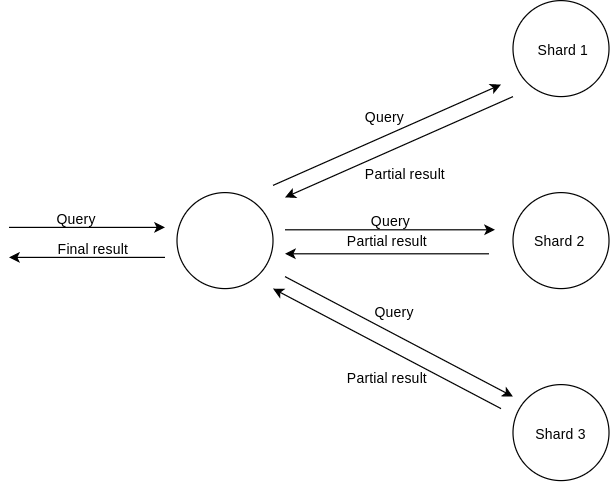
\includegraphics[width=0.9\linewidth]{img/elasticsearch-sharding.png}
  \caption{Elasticsearch distributing query agains all the shards}
  \label{fig:elasticsearch-sharding}
\end{figure}

\subsubsection{Aproximate Values}
As a result of Elasticsearch's distributed nature some queries will return estimated values.
Aggregations in Elasticsearch may return estimated values.

Table \ref{tbl:shard-term-counts} has a list of words across three different shards.
The term frequencies are listed inside the parenthesis.
When a client queries for the top three terms, the query is distributed to the shards.
Each shard then returns their local top three terms.
Given Table \ref{tbl:shard-term-counts},
the shards will return the terms listed in table \ref{tbl:shard-top}.
On the handler node [?? handler node] the global top three terms are calculated.
The top three terms is listed in table \ref{tbl:final-result}, which are \texttt{blue}, \texttt{sky} and \texttt{clouds}.
However, \texttt{blue}, \texttt{sky} and \texttt{clouds} are not the actual top three terms.
If the [?? handler] handler node had all the knowledge in table \ref{tbl:shard-term-counts},
the top three terms would be \texttt{blue}, \texttt{sky} and \texttt{insta},
with the term frequencies 60, 32 and 22 respectively.

[??] Write more here


\begin{table}[h!]
    \centering
    \begin{tabular}{|l|c|c|c|}
    \hline
    ~ & \textbf{Shard 1}    & \textbf{Shard 2}     & \textbf{Shard 3}    \\ \hline
    1 & blue (10)  & blue (20)   & blue (30)  \\ \hline
    2 & clouds (9) & clouds (12) & sky (25)   \\ \hline
    3 & sky (5)    & insta (5)   & insta (15) \\ \hline
    4 & plane (4)  & plane (3)   & plane (10) \\ \hline
    5 & insta (2)  & sky (2)     & rain (3)   \\ \hline
    \end{tabular}
    \caption{Term list with the corresponding term count.}
    \label{tbl:shard-term-counts}
\end{table}

\begin{table}[h!]
    \centering
    \begin{tabular}{|l|c|c|c|}
    \hline
    ~ & \textbf{Shard 1}    & \textbf{Shard 2}     & \textbf{Shard 3}    \\ \hline
    1 & blue (10)  & blue (20)   & blue (30)  \\ \hline
    2 & clouds (9) & clouds (12) & sky (25)   \\ \hline
    3 & sky (5)    & insta (5)   & insta (15) \\ \hline
    \end{tabular}
    \caption{Term list of the top three terms returned to the handler noder.[?? handler node]}
    \label{tbl:shard-top}
\end{table}

\begin{table}[h!]
    \centering
    \begin{tabular}{|l|c|}
    \hline
    ~ & \textbf{Returned result} \\ \hline
    1 & blue (60)     \\ \hline
    2 & sky (30)    \\ \hline
    3 & clouds (21)       \\ \hline
    \end{tabular}
    \caption{Top three terms which are returned back to the client.}
    \label{tbl:final-result}
\end{table}

https://www.elastic.co/guide/en/elasticsearch/reference/current/search-aggregations-bucket-terms-aggregation.html
